\subsection{Mineração}

Existe um outros serviços contidos dentro do projeto o \textit{dumont/specialist\_api} e \textit{dumont/specialist\_app} que gera uma API e uma interface gráfica para injeção de dados especialistas. Para subir ambos os serviços basta utilizar o comando \textit{docker-compose -f docker-compose.dev.yml up specialist\_app}. Entretanto, é necessário de um usuário para injetar as analises, é possível criar o documento na mão dentro do mongo, porem, existe um binário dentro da pasta chamado \textit{dumont/create\_specialist}, basta executa-lo passando o e-mail e ele te devolvera uma senha aleatória. Então basta acessar \textit{\url{http://127.0.0.1:3000/}} e utilizar os dados para entrar no sistema. Logo que autenticado você encontrara uma tela igual a da figura \ref{fig:specialist}, nela existe o tweet, uma área para adicionar perguntas da EADS relacionadas, e um local onde pode-se identificar palavras chaves dentro daquele tweet.

\begin{figure}
    \centering
    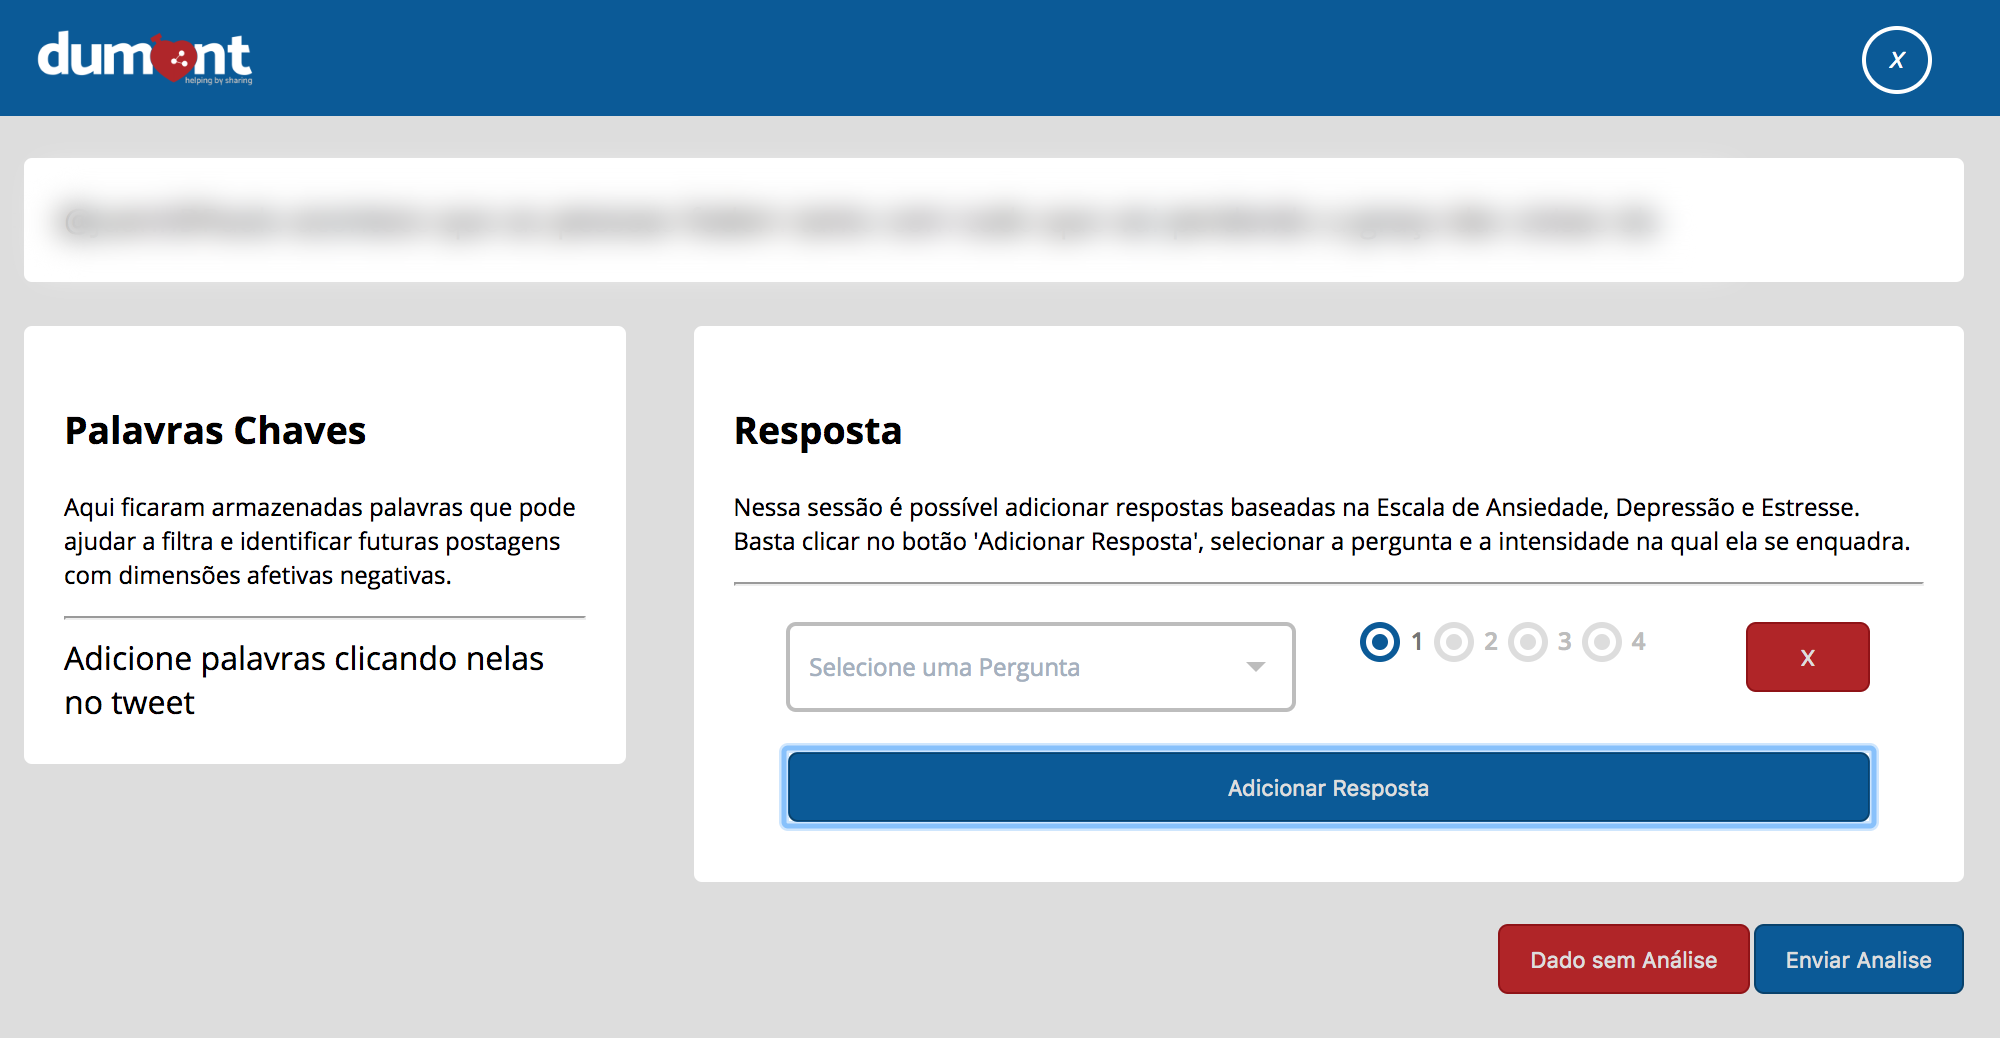
\includegraphics[width=1\textwidth]{imagens/specialist.png}
    \caption{Interface de captação de respostas dos especialistas}
    \label{fig:specialist}
\end{figure}

Com o sistema rodando, e dados sendo coletados e analisados é necessária uma amostragem para melhor assertividade e desenvolvimento. Durante a pesquisa, em uma preliminar foram coletados mais de 160GB de dados. A amostra foi tirada antes mesmo da inserção de dados especialistas, logo é necessário conhecer os \textit{scripts} de seleção do dumont.
